

\section{Elastic Attention}
\label{sec:method}
我们的方法概览见图~\ref{fig:method_main}。
子图~\ref{fig:method_main}(a) 展示了集成 Elastic Attention 模块后的整体结构，其核心为 Attention Router 机制。
需要强调的是，除 Elastic Attention 相关组件外，训练过程中骨干模型参数全部冻结。
% We describe our design from three perspectives below: Attention Router mechanism (\Cref{subsec:attention_router_mechanism}), training objective (\Cref{subsec:head_identification_optimization}), and efficient deployment (\Cref{subsec:deployment_of_attn_router}).

\begin{figure}[t]
  \centering
    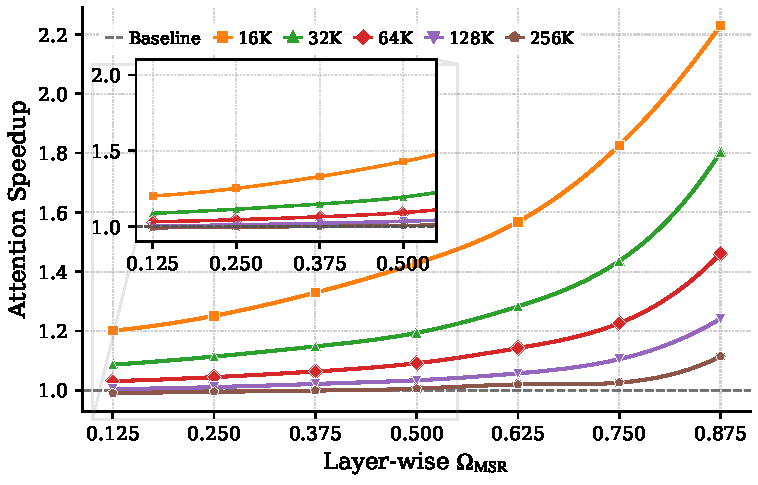
\includegraphics[width=\linewidth]{figures/kernel_speed.pdf}
    \caption{我们融合 kernel 与基于 Torch 的逐层串行混合注意力实现的速度对比。}
  \label{fig:kernel_speed_layerwise}
\end{figure}

\subsection{Attention Router 介绍}
\label{subsec:attention_router_mechanism}

\paragraph{Attention Router 的信息流}
如子图~\ref{fig:method_main}(b) 所示，Attention Router 的工作方式类似 Mixture-of-Experts（MoE）~\citep{shazeer2017outrageously} 门控：它根据输入隐状态，为每个 key-value 头分配注意力计算模式（FA 或 SA）。
具体来说，Key 隐状态（$\boldsymbol{x}_K\in\mathrm{\mathbb{R}^{s\times H\times d^{\prime}}}$，其中 $s$ 表示序列长度，$d^{\prime}$ 表示头维度）被送入 router。
随后，router 为每个头输出一个硬二值决策（$r_\mathrm{{hard}}^{(\ell,h)}\in \{0, 1\}$），表示该头采用 FA（$r_\mathrm{{hard}}^{(\ell,h)}=0$）还是 SA（$r_\mathrm{{hard}}^{(\ell,h)}=1$）。
每个头据此执行对应计算模式，最终在特征维拼接所有头输出，得到该层最终表示。

\paragraph{Attention Router 的结构设计}
子图~\ref{fig:method_main}(c) 展示了 router 结构，由两个组件组成：\textbf{task MLP} 与 \textbf{router MLP}。
task MLP 用于从输入隐状态中提取任务相关特征，router MLP 则基于该表示决定每个头的计算模式。
更具体地，给定 Key 隐状态（$\boldsymbol{x}_K$），router 先沿序列维进行池化，得到任务表示 $\boldsymbol{x}_K^{\prime}\in\mathrm{\mathbb{R}^{H\times d^{\prime}}}$。\footnote{实际中我们不在完整序列上池化，因为超长上下文包含大量冗余，可能降低任务表示质量。相关分析见附录~\ref{appdix:truncation_analysis}。}
再将池化后表示 $\boldsymbol{x}_K^{\prime}$ 输入 task MLP 与 router MLP，得到按头路由 logits 矩阵（$z\in\mathrm{\mathbb{R}^{H\times 2}}$），并通过 softmax 分类器转换为每个头的二值决策 $r_\mathrm{{hard}}^{(\ell,h)}$。

\subsection{基于优化的头识别}
\label{subsec:head_identification_optimization}

\paragraph{Attention Router 优化}
为保证训练与推理一致（推理使用硬路由，即二分类决策），我们在训练时同样采用硬路由。
这带来两个挑战：
(i) \emph{如何使 softmax 路由分布逼近硬路由决策}；
(ii) \emph{如何处理硬路由导致的不可导问题}。
针对第一个问题，我们采用带退火的 Gumbel--Softmax~\citep{jang2016categorical} 连续松弛策略，使路由分布在训练过程中逐步收敛到离散分配。
具体地，将 $z$ 输入 Gumbel--Softmax，得到软路由矩阵 $r^{(\ell)}_{\mathrm{soft}} \in \mathbb{R}^\mathrm{{H\times 2}}$，其中每列对应第 $\ell$ 层所有头的路由概率。
然后在第二维执行 $\arg\max$ 得到硬路由：
\begin{equation}
r_{\mathrm{hard}}^{(\ell,h)}
=
\mathop{\mathrm{argmax}}\limits_{c \in \{0,1\}} \; r_{\mathrm{soft}}^{(h,c)}, 
\qquad \forall h \in \{1,\dots,\mathrm{H}\}.
\end{equation}
针对第二个问题，由于 $\arg\max$ 不可导会阻断梯度，我们使用 straight-through estimator（STE）~\citep{bengio2013estimating}：
\begin{equation}
    r_{\mathrm{hard}}^{(\ell,h)} = r_{\mathrm{hard}}^{(\ell,h)} + \left[r_\mathrm{soft}^{(\ell,h)} - \mathrm{gradient\_detach}\left(r_\mathrm{soft}^{(\ell,h)}\right)\right],
\end{equation}
该写法使反向传播可通过软路由分布进行，同时前向仍保持硬路由行为。
更多细节与理论说明见附录~\ref{appdix:theoretical_explan_attn_router}。

\begin{table*}[t]
\centering
\caption{LongBench-E~\citep{bai2024longbench} 上的性能结果。我们报告各任务类别的平均性能（Perf.）与 $\Omega_{\mathrm{MSR}}$。
每个比较组中，性能第 1 与第 2 的结果分别以\textbf{加粗}和\underline{下划线}标出。
}
\resizebox{\textwidth}{!}{
\begin{tabular}{l | cc | cc | cc | cc | cc | cc | cc}
\toprule
\multirow{2}{*}{\textbf{方法}} & \multicolumn{2}{c|}{\textbf{S-Doc QA}} & \multicolumn{2}{c|}{\textbf{M-Doc QA}} & \multicolumn{2}{c|}{\textbf{Summ}} & \multicolumn{2}{c|}{\textbf{In-Context}} & \multicolumn{2}{c|}{\textbf{Synthetic}} & \multicolumn{2}{c|}{\textbf{Code}} & \multicolumn{2}{c}{\textbf{平均}} \\
\cmidrule(lr){2-3} \cmidrule(lr){4-5} \cmidrule(lr){6-7} \cmidrule(lr){8-9} \cmidrule(lr){10-11} \cmidrule(lr){12-13} \cmidrule(lr){14-15}
 & \textbf{性能} & $\mathbf{\Omega_{\mathrm{\bf MSR}}}$ & \textbf{性能} & $\mathbf{\Omega_{\mathrm{\bf MSR}}}$ & \textbf{性能} & $\mathbf{\Omega_{\mathrm{\bf MSR}}}$ & \textbf{性能} & $\mathbf{\Omega_{\mathrm{\bf MSR}}}$ & \textbf{性能} & $\mathbf{\Omega_{\mathrm{\bf MSR}}}$ & \textbf{性能} & $\mathbf{\Omega_{\mathrm{\bf MSR}}}$ & \textbf{性能} & $\mathbf{\Omega_{\mathrm{\bf MSR}}}$ \\
\arrayrulecolor{black}\midrule

% ==========================================
% SECTION 1: Qwen3-4B
% ==========================================
\rowcolor{blue!10}
\multicolumn{15}{c}{\textbf{Qwen3-4B 骨干模型}} \\
\arrayrulecolor{black!20}\midrule
Qwen3-4B & 43.69 & - & 38.48 & - & 28.46 & - & 66.21 & - & 49.59 & - & 54.38 & - & 48.45 & - \\
+ InfLLM-V2 & \underline{43.30} & - & 34.97 & - & \textbf{29.95} & - & 64.19 & - & 38.54 & - & \textbf{59.58} & - & 46.68 & - \\
+ DuoAttention & 41.73 & 0.70 & 35.72 & 0.70 & 28.47 & 0.70 & 64.59 & 0.70 & 47.17 & 0.70 & 53.91 & 0.70 & 46.95 & 0.70 \\
+ PruLong & 41.58 & 0.70 & 37.58 & 0.70 & \underline{28.53} & 0.70 & 64.80 & 0.70 & \underline{47.23} & 0.70 & 53.20 & 0.70 & 47.19 & 0.70 \\
\arrayrulecolor{black!40}\midrule
+ Elastic Attention (FA-SSA) & 42.20 & 0.66 & \underline{38.86} & 0.68 & 28.50 & 0.76 & \textbf{65.73} & 0.73 & \textbf{48.43} & 0.71 & \underline{54.34} & 0.82 & \textbf{48.08} & 0.73 \\
+ Elastic Attention (FA-XA) & \textbf{44.40} & 0.68 & \textbf{39.42} & 0.71 & 28.49 & 0.82 & \underline{65.26} & 0.76 & 44.35 & 0.74 & 54.29 & 0.87 & \underline{47.59} & 0.76 \\

% ==========================================
% SECTION 2: Qwen3-8B
% ==========================================
\arrayrulecolor{black}
\midrule
\rowcolor{blue!25}
\multicolumn{15}{c}{\textbf{Qwen3-8B 骨干模型}} \\
\arrayrulecolor{black!20}\midrule
Qwen3-8B & 45.57 & - & 51.59 & - & 28.34 & - & 66.64 & - & 50.16 & - & 61.20 & - & 52.16 & - \\
+ InfLLM-V2 & 42.20 & - & 42.33 & - & \textbf{29.58} & - & 64.55 & - & 45.87 & - & 59.58 & - & 49.03 & - \\
+ DuoAttention & 45.45 & 0.70 & 44.52 & 0.70 & 28.16 & 0.70 & 66.42 & 0.70 & 47.50 & 0.70 & \underline{62.38} & 0.70 & 50.67 & 0.70 \\
+ PruLong & \underline{46.05} & 0.70 & \underline{46.88} & 0.70 & \underline{28.30} & 0.70 & \underline{66.61} & 0.70 & \underline{48.66} & 0.70 & 62.24 & 0.70 & 51.34 & 0.70 \\
\arrayrulecolor{black!40}\midrule
+ Elastic Attention~(FA-SSA)& \textbf{46.15} & 0.64 & 46.54 & 0.65 & 28.19 & 0.72 & \textbf{67.52} & 0.71 & 48.07 & 0.65 & \textbf{62.95} & 0.78 & \underline{51.51} & 0.69 \\
+ Elastic Attention~(FA-XA)& 44.01 & 0.75 & \textbf{49.99} & 0.76 & \underline{28.30} & 0.83 & 66.23 & 0.80 & \textbf{50.95} & 0.77 & 60.57 & 0.86 & \textbf{51.66} & 0.80 \\

% ==========================================
% SECTION 3: Llama-3.1-8B
% ==========================================
\arrayrulecolor{black}
\midrule
\rowcolor{cyan!20}
\multicolumn{15}{c}{\textbf{Llama-3.1-8B-Instruct 骨干模型}} \\
\arrayrulecolor{black!20}\midrule
Llama-3.1-8B-Instruct & 48.75 & - & 51.85 & - & 30.26 & - & 68.16 & - & 56.00 & - & 55.81 & - & 53.28 & - \\
+ InfLLM-V2 & 43.77 & - & 46.30 & - & 30.08 & - & 67.32 & - & 42.03 & - & \textbf{64.30} & - & 50.73 & - \\
+ DuoAttention & 48.65 & 0.70 & 45.21 & 0.70 & 29.93 & 0.70 & 67.35 & 0.70 & \textbf{54.56} & 0.70 & 56.47 & 0.70 & 51.82 & 0.70 \\
+ PruLong & 47.69 & 0.70 & 43.05 & 0.70 & 30.02 & 0.70 & 67.86 & 0.70 & 53.56 & 0.70 & \underline{61.07} & 0.70 & 52.11 & 0.70 \\
\arrayrulecolor{black!40}\midrule
+ Elastic Attention~(FA-SSA)& \textbf{49.92} & 0.64 & \underline{48.92} & 0.63 & \underline{30.14} & 0.73 & \underline{67.99} & 0.74 & \underline{54.00} & 0.64 & 60.70 & 0.79 & \textbf{53.35} & 0.69 \\
+ Elastic Attention~(FA-XA)& \underline{49.40} & 0.71 & \textbf{52.94} & 0.69 & \textbf{30.30} & 0.80 & \textbf{68.55} & 0.79 & 49.66 & 0.72 & 56.49 & 0.87 & \underline{52.71} & 0.77 \\
% + Elastic Attention~(XA-SSA) & 48.30 & 0.63 & 46.40 & 0.62 & \underline{30.27} & 0.72 & 67.83 & 0.73 & 41.37 & 0.65 & \underline{60.81} & 0.78 & 50.71 & 0.69 \\

\arrayrulecolor{black}\bottomrule
\end{tabular}
}
\vspace{-0.5em}
\label{tab:longbench_main}
\end{table*}


\paragraph{训练目标}
训练时我们使用 $\Omega_{\mathrm{MSR}}$ 计算预测稀疏率，并与任务目标稀疏度 $\boldsymbol{t}$ 进行比较。
与为每个任务强制固定 $\boldsymbol{t}$ 不同，我们采用预设上下界的\emph{任务相关非紧约束}，因为单任务最优稀疏度通常未知。
为确保引入稀疏性后语言建模能力不下降，我们在标准语言建模目标上构造了带稀疏正则项的 min-max 优化目标。
给定输入 $\mathcal{X}$ 与标签 $\mathcal{Y}$，目标函数为：
\begin{equation}
\begin{aligned}
& \max_{\lambda_1, \lambda_2} \min \underbrace{L_{\mathrm{language}}(\mathcal{X})}_{\mathrm{language~modeling}} + \underbrace{\lambda_1 L_{\mathrm{diff}}(\mathcal{X}) + \lambda_2 L_{\mathrm{diff}}^{2}(\mathcal{X})}_{\mathrm{sparsity~regularization}}, \\
& \Rightarrow~\left\{
\begin{aligned}
& L_{\mathrm{language}} = \mathrm{CE\_Loss}\left(\mathcal{Y}\mid f_{\theta}(\mathcal{X})\right),\\
& L_{\mathrm{diff}} = \Omega_{\mathrm{MSR}}\left(f_\theta(\mathcal{X})\right) - \boldsymbol{t}, \
\end{aligned}
\right.
\end{aligned}
\label{equ:training_ojective}
\end{equation}
其中 $\mathrm{CE\_Loss}$ 是标准语言建模交叉熵损失，$\lambda_1, \lambda_2$ 为任务相关可训练拉格朗日乘子，通过梯度上升优化~\citep{bhaskar2025cache}，用于解耦不同任务间稀疏-性能权衡并缓解优化冲突。


\subsection{高效部署}
\label{subsec:deployment_of_attn_router}
由于每层都采用混合头计算，不同类型头在运行时难以高效并行，我们实现了融合注意力 kernel，以“同时”计算检索头与稀疏头。
本文聚焦单 GPU 部署，不引入设备间通信开销（如按头并行）。
在实现上，注意力 kernel 在序列维、注意力头维与 batch 维构成的三维网格上启动。
当输入序列足够长时，序列维并行主导整体执行。
由于并发 block 数受限于可用 streaming multiprocessor，GPU 实际上会先调度并执行某个头的大部分序列 block，再处理下一个头。
我们在图~\ref{fig:kernel_speed_layerwise} 中报告了相对基于 Torch 的串行逐层混合注意力实现的加速结果，表明融合 kernel 在推理 prefill 阶段能够带来加速。
更多细节见附录~\ref{appdix:deployment}。

% based on Block-Sparse-Attention~\citep{guo2024blocksparse}
% A natural concern is that sparse-head computation might be throttled by retrieval heads in the fused kernel. 
% Consequently, despite being conceptually independent, different heads are largely executed sequentially, and the observed speedup primarily stems from the reduced per-block computation of sparse heads.
